\documentclass[11pt, oneside]{article}   	% use "amsart" instead of "article" for AMSLaTeX format
\usepackage{geometry}                		% See geometry.pdf to learn the layout options. There are lots.
\geometry{letterpaper}                   		% ... or a4paper or a5paper or ... 
%\geometry{landscape}                		% Activate for for rotated page geometry
%\usepackage[parfill]{parskip}    		% Activate to begin paragraphs with an empty line rather than an indent
\usepackage{graphicx}				% Use pdf, png, jpg, or eps� with pdflatex; use eps in DVI mode
								% TeX will automatically convert eps --> pdf in pdflatex		
\usepackage{amssymb}
\usepackage{amsmath}
\usepackage{parskip}

\title{Substitutions for integration}
%\author{The Author}
\date{}							% Activate to display a given date or no date

\graphicspath{{/Users/telliott_admin/Dropbox/Tex/png/}}

\begin{document}

\maketitle
%\section{}
% \subsection*{R code}
% \begin{lstlisting}  \end{lstlisting}
% \begin{center} 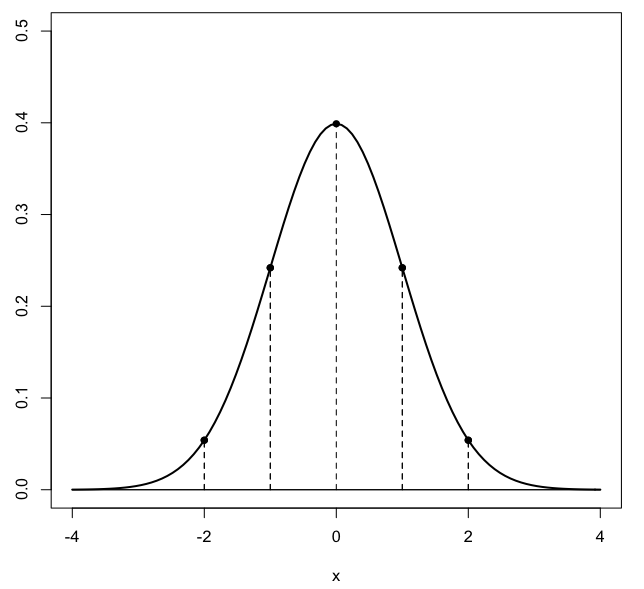
\includegraphics [scale=0.4] {gauss3.png} \end{center}
% \begin{bmatrix} a  &  b \\ c  &  d \end{bmatrix}
% \bigg |_

\Large
A "substitution" is a change of variable.  Suppose $f(x) = x^3$ and we want to do
\[ \int x^3 \ dx \]
We already know the answer to this because we know a function whose derivative is (within a constant multiplier and addend) equal to $f(x)$:
\[ \frac{d}{dx} \ x^4 = 4x^3 \]
If we integrate both sides of the equality we obtain
\[ \int \frac{d}{dx} \ x^4 = 4 \int x^3 \ dx \]
By definition the left-hand side is equal to $x^4$ so we have that:
\[ x^4 = 4 \int x^3 \]
plus a constant, of course.

We'll solve the same equation by substitution.  Let
\[ u = x^2, \ \ du = 2x \ dx \]
\[ \frac{1}{2} \ du = x \ dx \]
then 
\[  \int x^3 \ dx = \int x^2 \ x \ dx \]
\[ =  \frac{1}{2} \int u \ du \]
\[ = \frac{1}{4} \ u^2 \]
At this point we do the back substitution to convert back to $x$
\[ = \frac{1}{4} \ x^4 \]
Of course, you would never do this for such a simple integral, but it works, and it is the same basic idea.

There are two preeminent methods for differentiation:  the product (and quotient) rules, and the chain rule.  The substitution method is basically the reverse of the chain rule. 

Here is a problem where this idea really helps.  What is
\[ \int \tan x \ dx \]
\[ = \int \frac{\sin x}{\cos x} \ dx \]
This looks hard!  But what if we notice that the top is the derivative of what's on the bottom?  Then
\[ u = \cos x;  \ \ du = - \sin x \ dx \]
So we have 
\[ \int \frac{\sin x}{\cos x} \ dx = - \int \frac{1}{u} \ du \]
\[ = - \ln u \]
\[ = - \ln \cos x \]

Substitution allows us to see that we have both a function and its derivative inside the integral sign (when it may not be obvious, especially when you are first learning).
\[ \int x \ \cos(x^2 + 1) \ dx \]
With experience you won't need to do this, but here let
\[ u = x^2 + 1, \ \ du = 2x \ dx \]
\[ \frac{1}{2} \ du = x \ dx \]
then 
\[ \int x \ \cos(x^2 + 1) \ dx = \int \frac{1}{2} \ \cos u \ du \]
\[ = \frac{1}{2} \ \sin u \]
One crucial thing to remember is that for a definite integral, one must change the limits as well.
\[ \int_{x=0}^{x=2} x \ \cos(x^2 + 1) \ dx \rightarrow \int_{u=1}^{u=5}\ \frac{1}{2} \ \cos\ u \ du \]
Either that, or switch back to $x$ before evaluating.

Here is another example (also from wikipedia)
\[ \int_0^1 \sqrt{1-x^2} \ dx \]
Let
\[ x = \sin u, \ \ dx = \cos u \ du \]
then 
\[ \int_0^1 \sqrt{1-x^2} \ dx = \int \sqrt{1-sin^2\ u} \ \cos u \ du = \int \cos^2u \ du \]
Now, you may not know how to do this integral yet, but let me just make a couple of points.

1.  Before long, you will know this, it is $\frac{1}{2} (\sin u\ \cos u + u)$.
\vspace{2 mm} 

2.  We need to remember to switch the limits, which I skipped above.  Luckily $x$ goes from $0 \to 1$, so $u$ goes from $0 \to \pi/2$ to give the right result for $sin \ u$.  Plugging in
\[ \frac{1}{2} \ (\sin u\ \cos u + u) \bigg |_0^{\pi/2} = \frac{1}{2} \ \ \frac{\pi}{2} =  \frac{\pi}{4} \]

3.  If you look at the original function $\sqrt{1-x^2}$, this is just the equation of a unit circle, and we're integrating over the top right-hand quarter, so the result is just $\pi/4$.

Here are a few more examples.  
\[ \int \frac{x+1}{x^2 + 2x + 3} \ dx \]
Let
\[ t = x^2 + 2x + 3, \ \ dt = (2x + 2) \ dx, \ \ \frac{1}{2} dt = x + 1\]
\[ \int \frac{x+1}{x^2 + 2x + 3} \ dx = \frac{1}{2} \int \frac{1}{t} \ dt = \frac{1}{2} \ \ln t = \frac{1}{2} \ \ln (x^2 + 2x + 3) \]
\vspace{2 mm} 

\[ \int x \ e^{x^2} \ dx \]
let
\[ u = x^2, \ \ du = 2x \ dx \]
then  we have
\[ \int x \ e^{2x} \ dx \]
\[ = \frac{1}{2} \ \int e^u \ du \]
\[= e^u = e^{x^2}  \]

Last, a very common type of problem:

\[ \int x \sqrt{2x + 1} \ dx \]

Any time we have the integral of $x$ times some function $f(x)$ it will be based on the product rule:
\[ (uv)' = uv' + u'v \]
Integrating
\[ uv = \int uv' + \int u'v \]
\[ \int uv' = uv - \int u'v \]
where $u(x)$ is just $x$.

To put it another way, we are going have something like $x$ times the integral of the rest of it (that's the $uv$), and then a correction term (that's the $\int u'v$ part).

We could guess.  What is
\[ \frac{d}{dx} \ [ \ x (2x+1)^{3/2} \ ] = ? \]
From the product rule:
\[ = 3 x (2x+1)^{1/2} + (2x+1)^{3/2} \]
Correct for the factor of $3$
\[ \frac{d}{dx} \ [\ \frac{1}{3}x (2x+1)^{3/2} \ ] = ? \]
\[ = x (2x+1)^{1/2} + \frac{1}{3}(2x+1)^{3/2} \]
We have what we want in the first term.  We just need a correction factor to make the second term go away.  We need something that when we take the derivative we get minus that term.
\[ \int \frac{1}{3}(2x+1)^{3/2} = \frac{n}{d} (2x+1)^{5/2}\]
The only trick is to get the fraction right so as to cancel what comes down from the exponent, and what comes from the $2x + 1$ term inside.  The correct answer is
\[  \frac{1}{15} (2x+1)^{5/2}\]
and putting it all together we obtain
\[ \frac{1}{3}x (2x+1)^{3/2} - \frac{1}{15} (2x+1)^{5/2}\]
This can be simplified a bit, but let's wait.

Rather than guess, we can use two systematic approaches.  The first is substitution (which is why the problem is in this unit), and the other is integration by parts, which basically formalizes the guessing approach that we took above.

Here is the substitution method.  Our problem is:
\[ \int x \sqrt{2x + 1} \ dx \]

Let $u = 2x + 1$, then $x = (u-1)/2$ and $du = 2 dx$ so we obtain
\[ \frac{1}{2} \int \frac{(u-1)}{2} \sqrt{u} \ du \]
\[ = \frac{1}{4} \ [ \ \int u^{3/2} \ du - \int u^{1/2} \ du \ ] \]
\[ = \frac{1}{4} \ [ \ \frac{2}{5}u^{5/2} - \frac{2}{3}u^{3/2} \ ] \]
\[ = \frac{1}{2} \ [ \ \frac{1}{5}(2x + 1)^{5/2} - \frac{1}{3} (2x + 1)^{3/2} \ ] \]
Comparing with what we had above, it doesn't look like the same answer.  Let's try rearranging by factoring out the $3/2$ power:

\[ = \frac{1}{2}(2x + 1)^{3/2} \ [ \ \frac{1}{5}(2x + 1) - \frac{1}{3} \ ] \]
\[ = \frac{1}{2}(2x + 1)^{3/2} \ [ \ \frac{2}{5}x - \frac{2}{15} \ ] \]
\[ = (2x + 1)^{3/2} \ [ \ \frac{1}{5}x - \frac{1}{15} \ ] \]
whereas the original answer was
\[ \frac{1}{3}x (2x+1)^{3/2} - \frac{1}{15} (2x+1)^{5/2}\]
and factoring, we get
\[ = (2x+1)^{3/2} \ [ \ \frac{1}{3}x - \frac{1}{15}(2x + 1) \ ] \]
\[ = (2x+1)^{3/2} \ [ \ \frac{1}{5}x -\frac{1}{15} \ ] \]
which checks.

\end{document}  